\begin{frame}
    % \par Different board examples:
    \begin{columns}
        \begin{column}{0.5\textwidth}
            \begin{figure}
                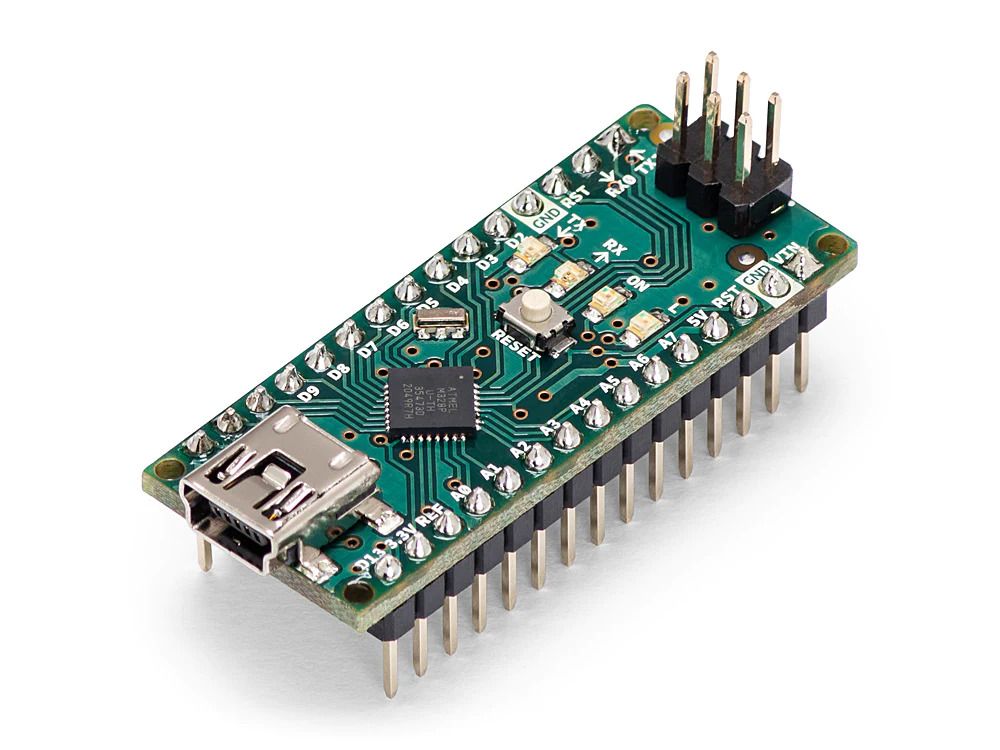
\includegraphics[height=2cm]{microcontroller/arduino/boards/nano.jpg}
                \caption{Arduino\textregistered{} Nano (\textit{Nano Family})}
            \end{figure}
            \begin{figure}
                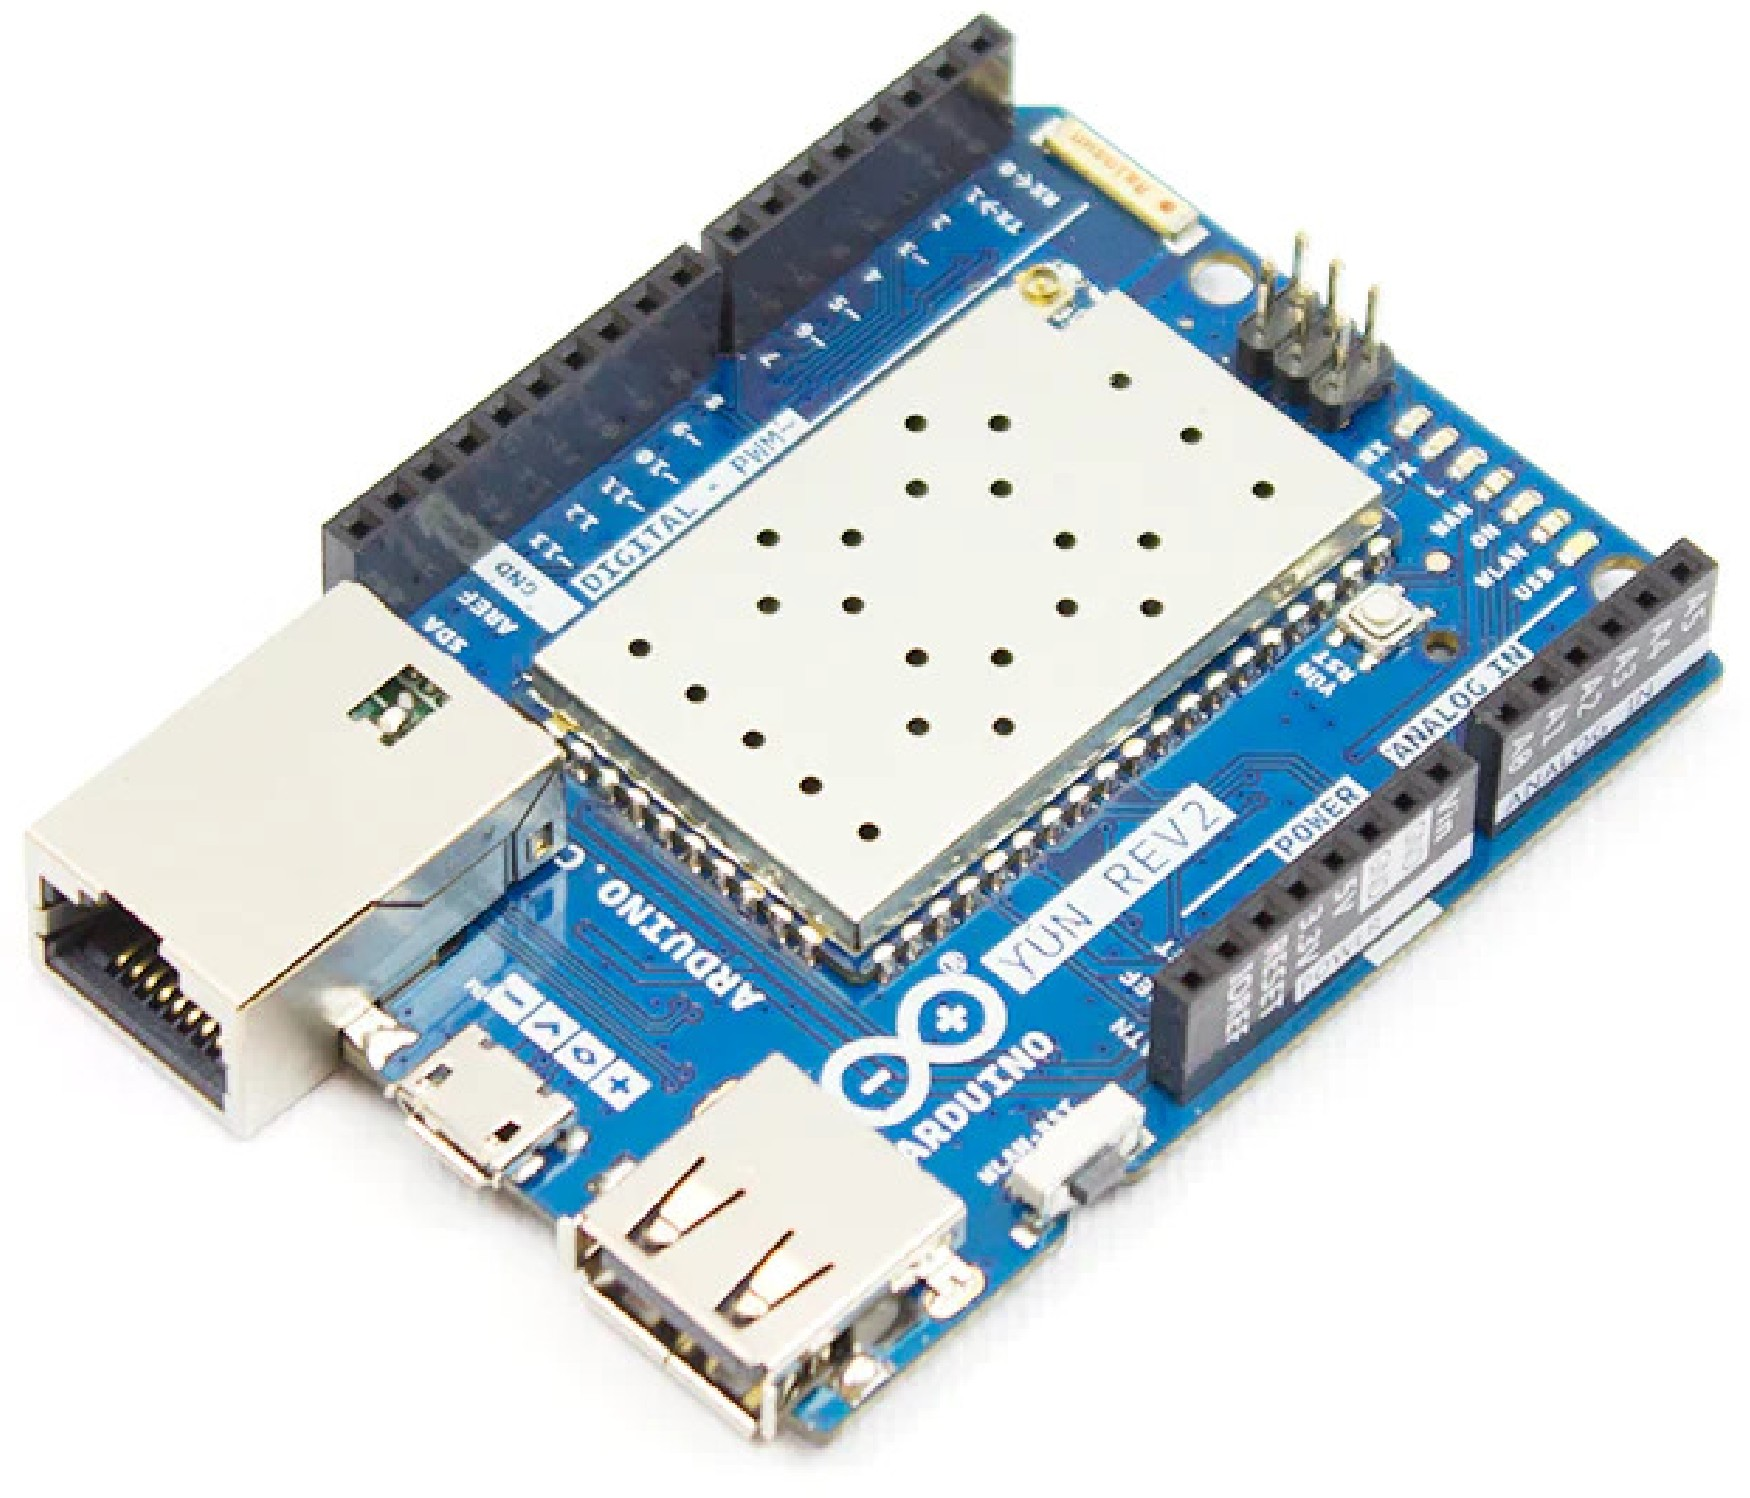
\includegraphics[height=2.7cm]{microcontroller/arduino/boards/yun.jpg}
                \caption{Arduino\textregistered{} Yún (\textit{Classic})}
            \end{figure}
        \end{column}
        \begin{column}{0.5\textwidth}
            \begin{figure}
                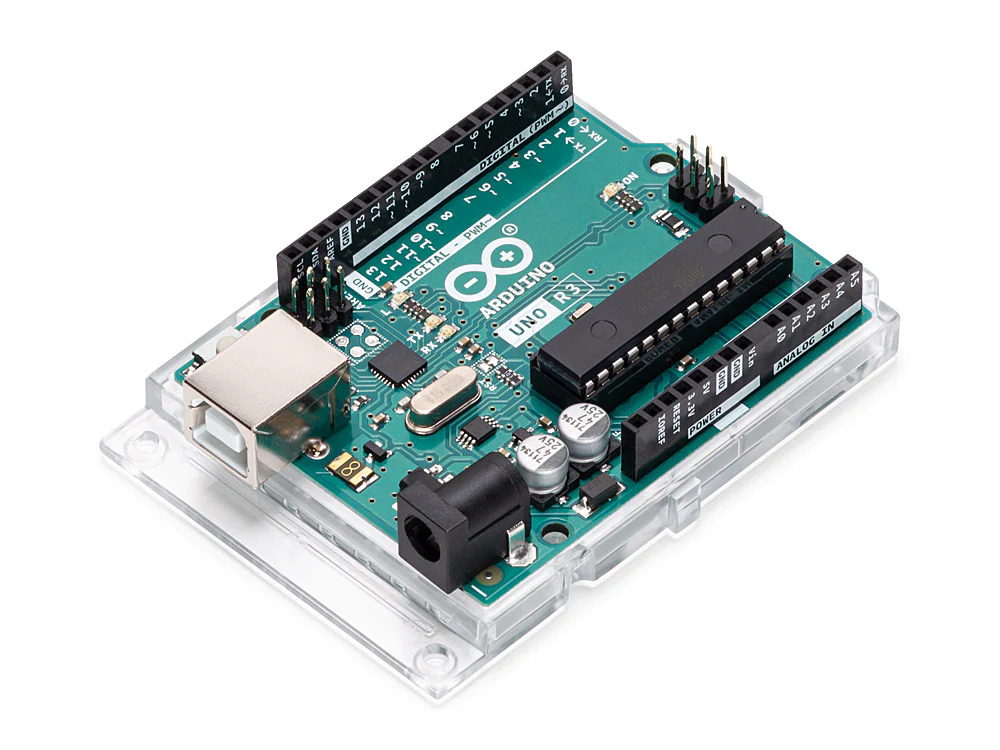
\includegraphics[height=2.7cm]{microcontroller/arduino/boards/uno.jpg}
                \caption{Arduino\textregistered{} Uno (\textit{Classic})}
            \end{figure}
            \begin{figure}
                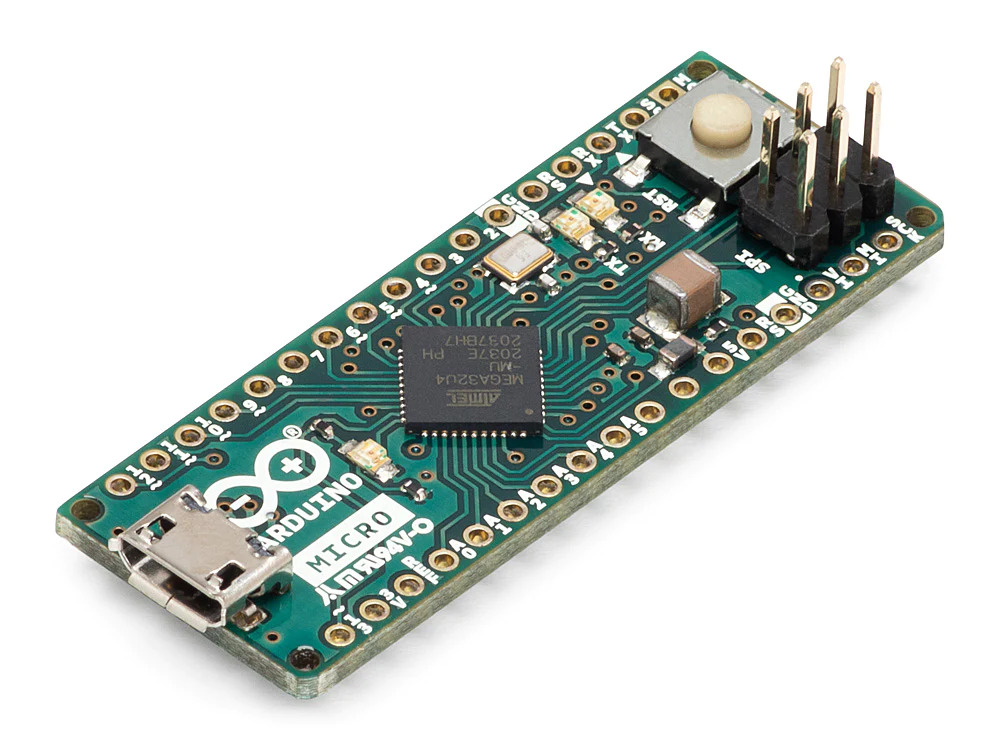
\includegraphics[height=2cm]{microcontroller/arduino/boards/micro.jpg}
                \caption{Arduino\textregistered{} Micro (\textit{Classic})}
            \end{figure}
        \end{column}
    \end{columns}
\end{frame}

\begin{frame}
    % \par Different board examples:
    \begin{columns}
        \begin{column}{0.5\textwidth}
            \begin{figure}
                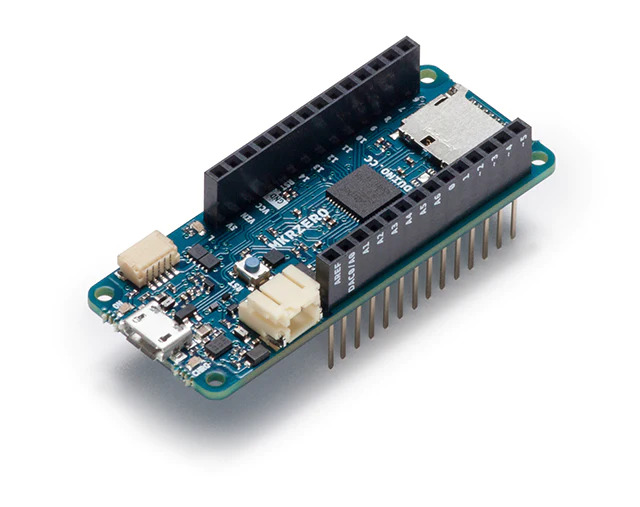
\includegraphics[height=2cm]{microcontroller/arduino/boards/mkr-zero.jpg}
                \caption{Arduino\textregistered{} MKR ZERO (\textit{MKR Family})}
            \end{figure}
            \begin{figure}
                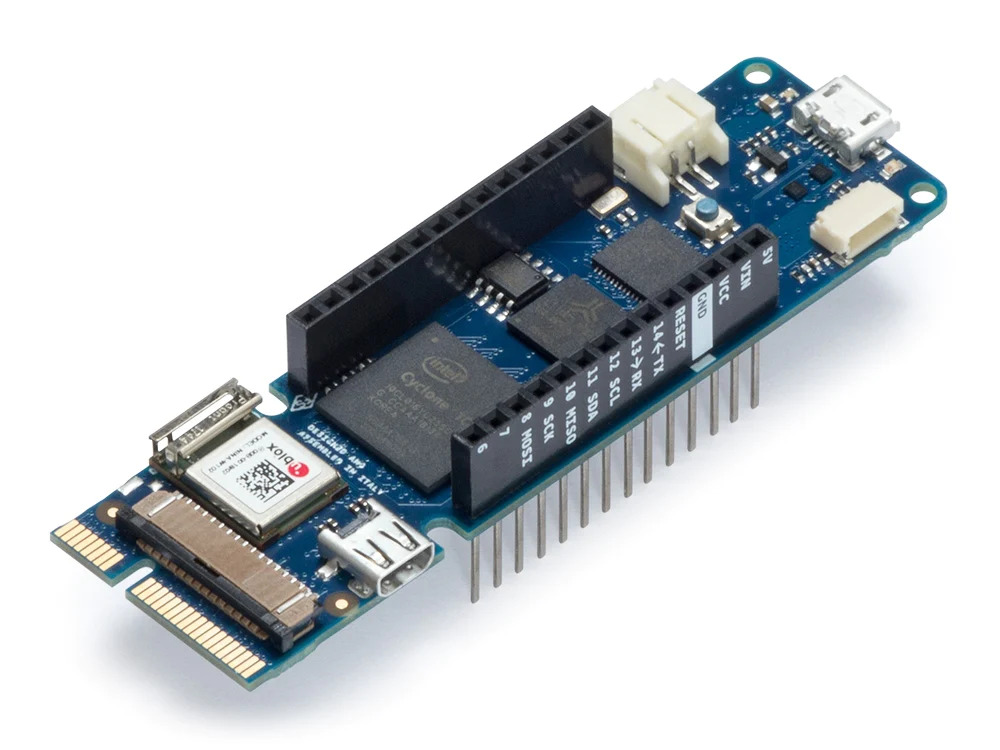
\includegraphics[height=2cm]{microcontroller/arduino/boards/mkr-vidor-4000.jpg}
                \caption{Arduino\textregistered{} MKR Vidor 4000 (\textit{MKR Family})}
            \end{figure}
        \end{column}
        \begin{column}{0.5\textwidth}
            \begin{figure}
                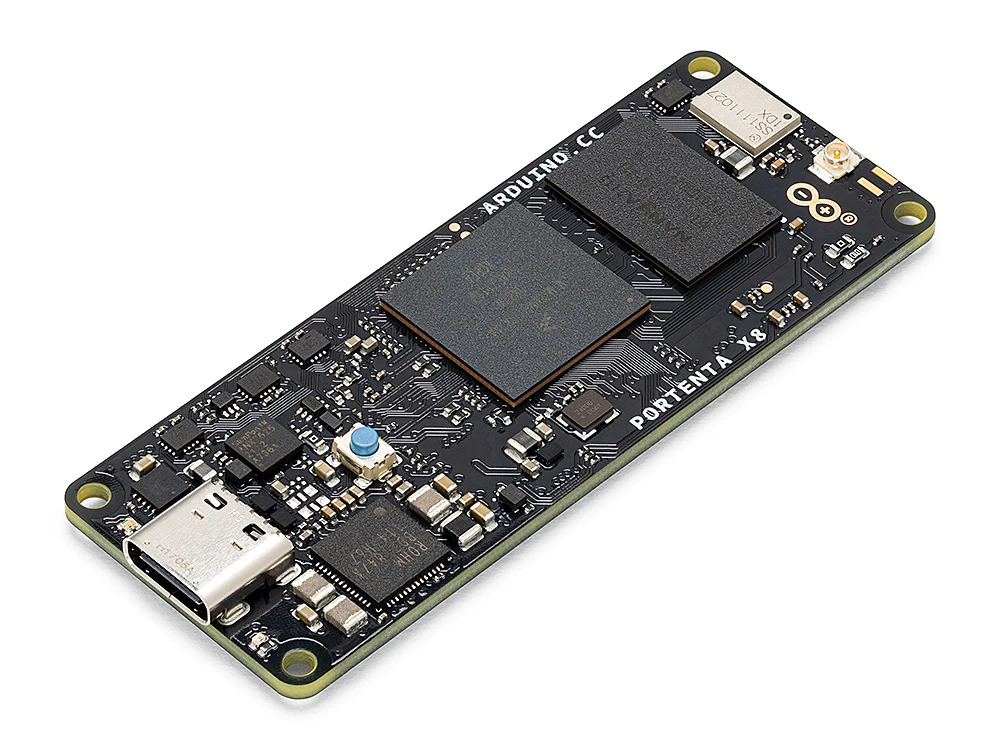
\includegraphics[height=2cm]{microcontroller/arduino/boards/portenta-x8.jpg}
                \caption{Arduino\textregistered{} Portenta X8 (\textit{Portenta Family})}
            \end{figure}
            \begin{figure}
                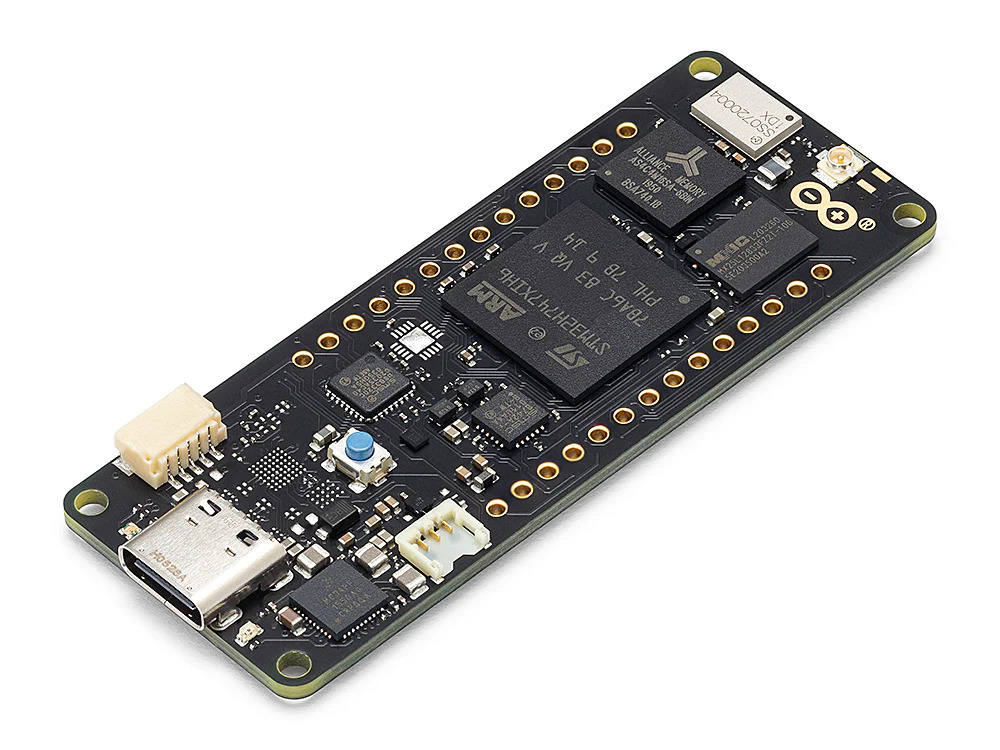
\includegraphics[height=2cm]{microcontroller/arduino/boards/portenta-h7-lite-connected.jpg}
                \caption{Arduino\textregistered{} Portenta H7 Lite Connected (\textit{Portenta Family})}
            \end{figure}
        \end{column}
    \end{columns}
\end{frame}
